\hypertarget{cross-track-ties-and-the-one-grammar-thesis}{%
\section{Cross-track ties, and the one-grammar thesis}\label{cross-track-ties-and-the-one-grammar-thesis}}

The per-track results stand on their own. But the calculus offers something that neither track shows alone and that, to
our knowledge, no other framework in either domain produces: \textbf{the same structural object turning out to be two
different physical phenomena}, on substrates that share no physics. These cross-track ties are not analogies or shared
tooling --- they are single objects in one grammar, read on two substrates that were explicitly guarded against each
other. We catalog them first (§8.2), argue why they are distinctive rather than coincidental (§8.3), and then draw the
thesis they support (§8.4).

\hypertarget{why-the-ties-are-non-trivial-the-anti-contamination-guard}{%
\subsection{Why the ties are non-trivial: the anti-contamination guard}\label{why-the-ties-are-non-trivial-the-anti-contamination-guard}}

The evidential weight of ``one object, two phenomena'' collapses if the two constructions were allowed to copy each
other. They were not. An \textbf{anti-contamination protocol} was declared at the outset: the SM substrate is a
\emph{selection/measure} layer (\(P_2\)-dominant --- a candidate space, constraints, a measure); the QM--GR substrate is a
\emph{co-sourcing common refinement} (\(P_4\)/F51 --- one field, two readouts). Build validators on the SM track fail on any
field-carrier token; steps that pattern-matched one substrate onto the other were rejected during construction
(Section 3.4). So when a single object surfaces on both tracks, it is because the \emph{law} is layer-agnostic --- not because
one construction borrowed from the other. Every tie below survived that guard.

\hypertarget{the-cross-track-ties}{%
\subsection{The cross-track ties}\label{the-cross-track-ties}}

\begin{quote}
\textbf{Each row is one object, computed on both substrates.} Read across: the leftmost column is a single construct of the
calculus; the next two columns are what it \emph{is} on each track.
\end{quote}

\begin{longtable}[]{@{}lll@{}}
\toprule
\begin{minipage}[b]{0.23\columnwidth}\raggedright
one calculus object\strut
\end{minipage} & \begin{minipage}[b]{0.35\columnwidth}\raggedright
on the SM substrate (selection layer)\strut
\end{minipage} & \begin{minipage}[b]{0.35\columnwidth}\raggedright
on the QM--GR substrate (common refinement)\strut
\end{minipage}\tabularnewline
\midrule
\endhead
\begin{minipage}[t]{0.23\columnwidth}\raggedright
\textbf{factorization defect} \(\Delta_{\mathrm{fact}}\)\strut
\end{minipage} & \begin{minipage}[t]{0.35\columnwidth}\raggedright
the \(X/Y\) colored coset --- proton decay, monopole, color-separation, GUT non-relabeling, one object (§4.4)\strut
\end{minipage} & \begin{minipage}[t]{0.35\columnwidth}\raggedright
the ladder defect (\(8\) witnesses) + the route-mismatch \(\Delta_3^{\mathrm{comp}}\) --- \emph{non-renormalizability} (§5.1--5.2)\strut
\end{minipage}\tabularnewline
\begin{minipage}[t]{0.23\columnwidth}\raggedright
\textbf{the record / memory rung}\strut
\end{minipage} & \begin{minipage}[t]{0.35\columnwidth}\raggedright
grounds clean-separation, \emph{forbids proton decay \& monopoles} (Pred. 3); hosts the measurement discriminator\strut
\end{minipage} & \begin{minipage}[t]{0.35\columnwidth}\raggedright
grounds the common carrier; makes the gravitational channel a record channel --- \emph{forbids BMV entanglement} (Pred. 2)\strut
\end{minipage}\tabularnewline
\begin{minipage}[t]{0.23\columnwidth}\raggedright
\textbf{F51 common refinement}\strut
\end{minipage} & \begin{minipage}[t]{0.35\columnwidth}\raggedright
the GUT parent → \(\sin^2\theta_W = 3/8\), \(k_Y = 5/3\) (trace ratios)\strut
\end{minipage} & \begin{minipage}[t]{0.35\columnwidth}\raggedright
the parent \(L\) → fork-over-ladder; forces the monogamy combiner\strut
\end{minipage}\tabularnewline
\begin{minipage}[t]{0.23\columnwidth}\raggedright
\textbf{GROUND landing mode}\strut
\end{minipage} & \begin{minipage}[t]{0.35\columnwidth}\raggedright
clean-separation \(\leftarrow\) record-stability\strut
\end{minipage} & \begin{minipage}[t]{0.35\columnwidth}\raggedright
common carrier \(\leftarrow\) semiclassical co-sourcing\strut
\end{minipage}\tabularnewline
\begin{minipage}[t]{0.23\columnwidth}\raggedright
\textbf{F37 complementarity} (non-joint-access)\strut
\end{minipage} & \begin{minipage}[t]{0.35\columnwidth}\raggedright
(the access-quotient discipline of the selection layer)\strut
\end{minipage} & \begin{minipage}[t]{0.35\columnwidth}\raggedright
the premise controls (no joint quotient for non-commuting accesses); reconciles the carrier with Bell (§7.1)\strut
\end{minipage}\tabularnewline
\begin{minipage}[t]{0.23\columnwidth}\raggedright
\textbf{F47/F26 demarcation} (no value-law on contingent selection)\strut
\end{minipage} & \begin{minipage}[t]{0.35\columnwidth}\raggedright
no value-law on the EW scale, \(N_{\mathrm{gen}}\), content\strut
\end{minipage} & \begin{minipage}[t]{0.35\columnwidth}\raggedright
no in-layer \(\Lambda\) value-law (F50 bounded-moduli, §7.3)\strut
\end{minipage}\tabularnewline
\bottomrule
\end{longtable}

Three of these are physical statements, not bookkeeping:

\begin{itemize}
\item
  \textbf{One defect is both proton physics and non-renormalizability.} \(\Delta_{\mathrm{fact}}\) --- the failure of one
  readout to factor through another --- is, on the SM substrate, the \(X/Y\) coset whose \emph{absence} makes the proton stable;
  on the QM--GR substrate, it is the obstruction that makes quantizing gravity fail. The calculus says these two
  century-old difficulties are the \emph{same kind of structural fact} about layered descriptions, surfacing on different
  substrates.
\item
  \textbf{One rung underlies three of the paper's headline results.} Record/memory stability --- the requirement that a
  universe be able to hold stable records --- grounds the SM gauge selection (§4.5), forbids proton decay (Prediction 3),
  \emph{and} forces the gravitational channel to be a record channel that decoheres without entangling (Prediction 2). A
  single structural commitment, stated once, has consequences in particle physics \emph{and} in tabletop gravity. This is
  the most consequential tie: it predicts that \emph{whatever forbids the proton from decaying is the same structure that
  prevents gravity from entangling masses} --- a connection no separate treatment of the two would suggest.
\item
  \textbf{One refinement law lands a gauge angle and resolves quantum gravity's architecture.} F51 (unification as common
  refinement) builds the GUT parent that yields \(\sin^2\theta_W = 3/8\) on one substrate and the QM--GR parent that
  selects the fork on the other --- the same commuting-square construction, two unrelated payoffs.
\end{itemize}

\hypertarget{why-this-is-distinctive-and-not-coincidence}{%
\subsection{Why this is distinctive --- and not coincidence}\label{why-this-is-distinctive-and-not-coincidence}}

Two reasons these ties are evidence rather than wordplay. First, \textbf{the anti-contamination guard} (§8.1): the objects
recur across substrates that were prevented from sharing structure, so the recurrence is forced by the laws. Second,
\textbf{the ties do work} --- each is load-bearing in a \emph{result}, not decorative: the shared record rung is what lets
Predictions 2 and 3 use one record constraint without collapsing their distinct physical claims; the shared \(\Delta_{\mathrm{fact}}\) is what lets the
non-renormalizability typing and the proton-stability spine be checked by one piece of frozen machinery. A coincidence
of notation could do neither.

This is, we contend, a distinctive feature of a layer-agnostic calculus, and one not easily reproduced by
domain-specific methods: a quantum-gravity framework has no reason to predict proton stability, and a
grand-unified model has no reason to constrain gravitationally-induced entanglement, but a calculus whose objects are
substrate-independent \emph{forces} such links and states them as predictions (§6).

\hypertarget{the-one-grammar-thesis}{%
\subsection{The one-grammar thesis}\label{the-one-grammar-thesis}}

The ties support a single claim --- the thesis of the foundations program (visible in the title of its law catalog:
\emph{layer-agnostic} structural laws):

\begin{quote}
\textbf{One frozen grammar --- quotients, closures, descent, factorization defects, common refinements, fiber volumes,
landing modes --- applied to the two most structurally unrelated deep problems in physics, produced foundational-grade
results on both, in the two opposite genres its own laws anticipated in advance, tied them through shared structural
objects, and yielded three falsifiable mainstream-contradicting predictions.}
\end{quote}

Layer-agnosticism cannot be tested on one substrate; it is tested by freezing the grammar and pointing it at problems
that share nothing --- a deliberately conducted \(n=2\) experiment. And the result was not indiscriminate success but
\textbf{differential, predicted success}: the framework's own laws assign the two problems \emph{different expected genres}.
F47/F26 say a \textbf{contingent selection} supports no value-law --- so the SM track should yield demarcations, blindness
theorems, and conditional selections, with its value-law attempts failing or landing only as embedding ratios. A
\textbf{co-sourcing refinement} supports a positive relation between its two readouts --- so the QM--GR track is where an
\(E=mc^2\)-shaped law could land. Both expectations were recorded \emph{before} the corresponding constructions ran (the
value-law push was explicitly parked on the SM track and redirected to QM--GR on exactly this reasoning), and both were
borne out: the SM track delivered the demarcation profile (including the failures of its value-law attempts), the
QM--GR track landed the ledger/shadow-price relation (review-settled). The grammar \textbf{forbids different things in
different places, and its successes and failures fell along its own forbidding} --- the signature of a meta-theory with
content, not a flexible vocabulary. The three falsifiable predictions then arose from the same final move applied to
each track's strongest theorem, under the same symmetric-scrutiny discipline.

\hypertarget{the-honest-bound-on-the-thesis}{%
\subsection{The honest bound on the thesis}\label{the-honest-bound-on-the-thesis}}

\begin{itemize}
\tightlist
\item
  \(n=2\) is evidence, not proof, of layer-agnosticism; the atlas of foreclosures contains dozens of further edges, each
  a test the thesis could fail.
\item
  Both substrates are finite toys; frame-transfer is unproven on both. The grammar's universality is demonstrated at
  the level of \emph{structure recovered, demarcated, tied, and predicted} --- not of nature derived.
\item
  The construction program was adversarially reviewed at both ends --- two QM--GR bundles settled and the SM core passed
  review --- but has not been independently replicated; the §6 predictions await independent review.
\item
  The ties are structural identities \emph{within the calculus}; we do not claim the SM and quantum gravity are ``the same
  physics'', only that one structural grammar describes both and links them --- and that the links are falsifiable
  (Predictions 2--3 are the shared record rung made testable).
\end{itemize}

\begin{figure}[tbp]
  \centering
  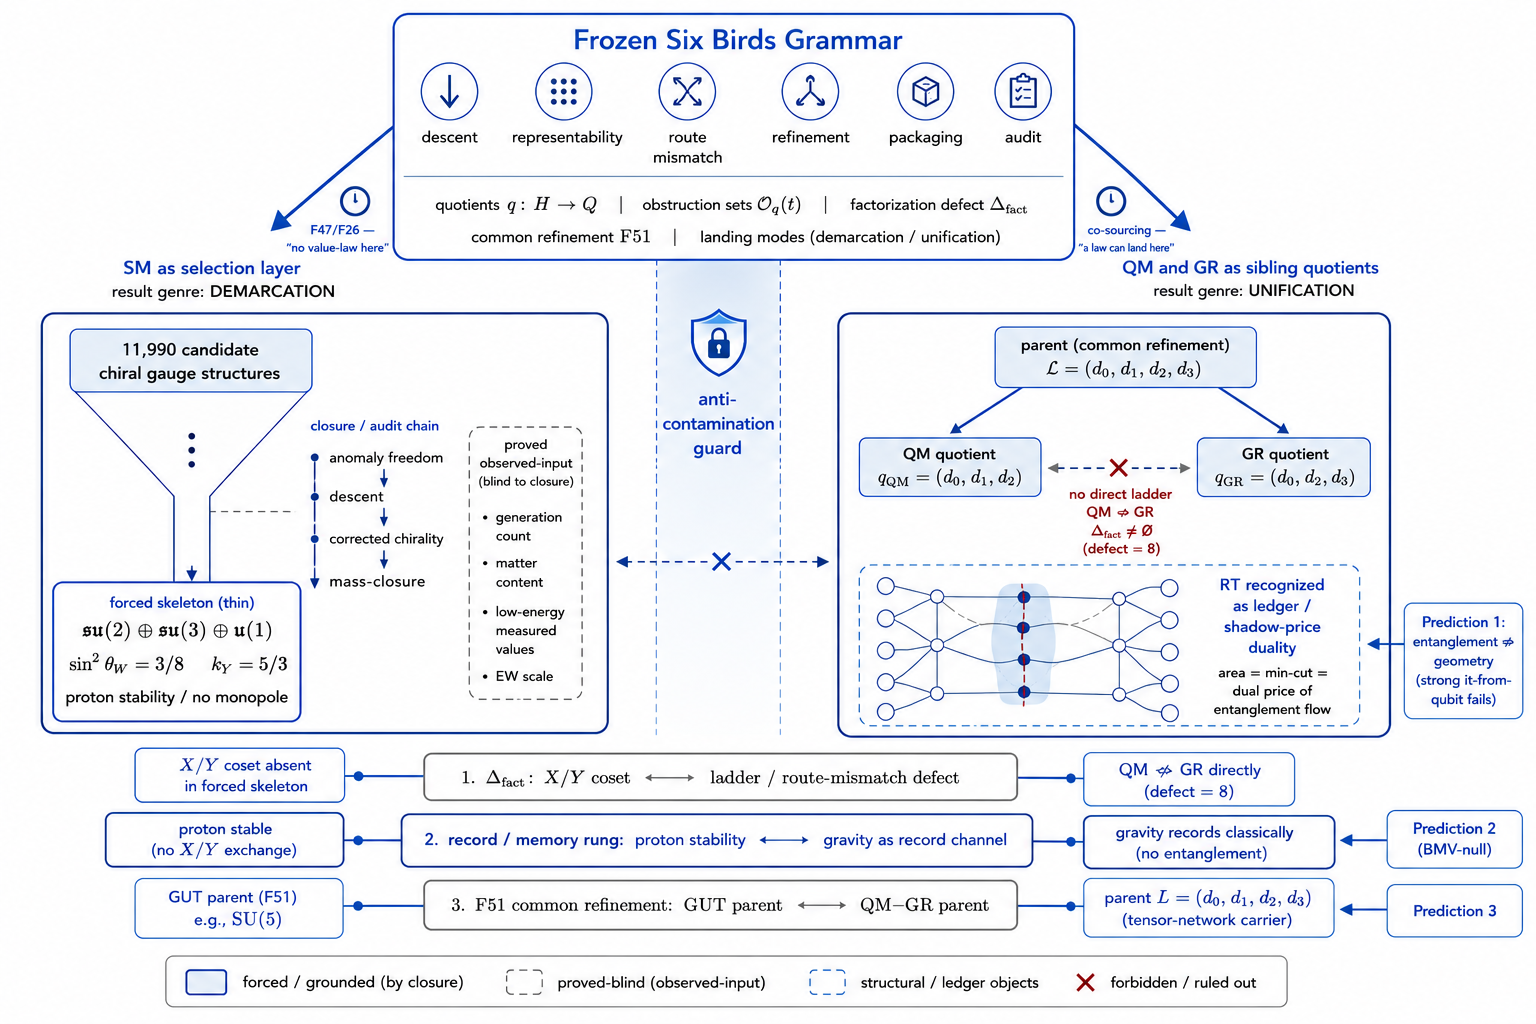
\includegraphics[width=\linewidth]{figures/fig_f1_one_grammar.png}
  \caption{\textbf{The paper's thesis in one panel.} \emph{Center: the grammar (six primitives + F-laws, one box). Two arrows out, through an ``anti-contamination guard'' wall: left to the SM substrate (selection layer) yielding the demarcation stack (§4) and Prediction 3; right to the QM--GR substrate (common refinement) yielding the unification stack (§5) and Predictions 1--2. Beneath each arrow, the prior expectation (F47/F26: ``no value-law here''; co-sourcing: ``a law can land here'') with a timestamp glyph indicating the expectation preceded the result. Connecting the two arms: the cross-track ties of §8.2 drawn as rungs between the substrates --- labeled \(\Delta_{\mathrm{fact}}\), the record rung, F51 --- with the record rung highlighted as the spine of Predictions 2 and 3.}}
  \label{fig:f1}
\end{figure}
